\chapter{Introduction}
\label{chap:Introduction}

In absence of the right-handed neutrino fields, the renormalizable Standard Model (SM) Lagrangian exhibits a few continuous global symmetries, namely the U(1)$_{\text{L}_{i}}$ that give rise to the conservation of lepton family numbers. Unlike gauge symmetries of the SM, which arise at the outset of the construction, these global U(1) symmetries emerge accidentally due to the assumption (massless neutrino) that is solely driven by phenomenology. Despite the accidental nature of these symmetries, they have stood up to the tests of almost all particle physics experiments to date.  

\begin{figure}[tbh!]
 \begin{center}
 \begin{tabular}{c}
 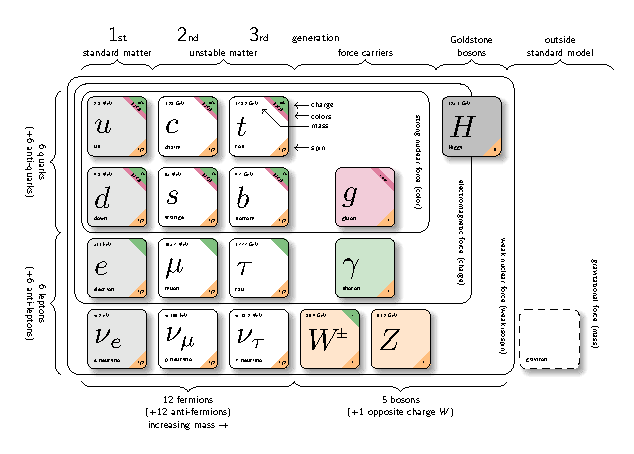
\includegraphics[width=\textwidth]{figures/SM}
 \end{tabular}
 \caption{The field content of the \ac{SM}, including all known elementary particles. The three generations of fermions are shown in the first three columns. The gauge bosons that mediate the fundamental interactions are shown in fourth and fifth columns. The sixth column shows the recently discovered Higgs boson. The hypothetical graviton that mediates gravitational force is also shown, which is outside of realm of the \ac{SM}.~\cite{tikz:SM}}
 \label{fig:5fold}
 \end{center}
\end{figure}

In absence of the right-handed neutrino fields, the renormalizable Standard Model (SM) Lagrangian exhibits a few continuous global symmetries, namely the U(1)$_{\text{L}_{i}}$ that give rise to the conservation of lepton family numbers. Unlike gauge symmetries of the SM, which arise at the outset of the construction, these global U(1) symmetries emerge accidentally due to the assumption (massless neutrino) that is solely driven by phenomenology. Despite the accidental nature of these symmetries, they have stood up to the tests of almost all particle physics experiments to date.  

In fact, the first and so far the only hint of the broken global symmetries didn't appear until the turn of the century through the oscillation of atmospheric neutrinos \cite{Super-Kamiokande:1998kpq,SNO:2002tuh}. This remarkable observation directed significant interest from both theorists and experimentalists to the flavor sector of the SM. On the one hand, it cements the calls for extensions of the SM by demonstrating the mixing of neutrino flavors. On the other hand, it also suggests that the U(1)$_{\text{L}_{i}}$ symmetries are indeed broken, and the charged lepton flavor violation (CLFV) should also occur. 

Although the exact mechanism behind neutrino mass remains unclear, it can be induced through two distinct ways that only require minimal departures from the original formulation of the SM. By adding right-handed neutrino fields, the Yukawa coupling \cite{PhysRevLett.19.1264} that describes the emergence of Dirac fermion masses can be naturally extended to neutrinos. The neutrino mass can also be realized by introducing the nonrenormalizable Dimension-5 operator \cite{Weinberg:1979sa}, known as the Weinberg operator. This operator gives rise to Majorana neutrino mass terms upon spontaneous symmetry breaking. 

In either case, the masses of neutrinos are accounted for and the strength of the neutrino flavor mixing is governed by the PMNS matrix \cite{Pontecorvo:1957cp,Maki:1962mu}, a nearly perfect analog to the CKM matrix \cite{Cabibbo:1963yz,Kobayashi:1973fv} that describes quark mixing in the weak interaction. The same PMNS matrix can also give rise to the CLFV process through loop diagrams involving charged current. However, these diagrams are highly suppressed and phenomenologically negligible due to the small neutrino mass relative to the electroweak scale. Therefore, any experimental observation of CLFV will be unambiguous evidence of new physics beyond the SM.

reported by the LHCb experiment mark the first major deviation from the SM produced by the Large Hadron Collider (LHC). Not only did this result provide a direct hint towards lepton flavor universality violation (LFUV), it also prompted renewed experimental interest in CLFV search since models that accommodate LFUV generally give rise to LFV as well \cite{Glashow:2014iga}. The LHC provides the best sensitivity to CLFV processes involving a heavy leg, such as a top quark or a Higgs boson. Moreover, some of these models \cite{Kim:2018oih} also suggest that CLFV involving a top quark is within the reach of the LHC sensitivity. Therefore, a search for CLFV in the top quark sector could shed light on these flavor anomalies and further our understanding of the broken global symmetries.

This thesis describes the research work I did in 2019-2023 on the \ac{CMS} experiment, including a brief description of the surrounding context and background knowledge. This thesis is organized into four parts, and \autoref{Part1} introduces the theoretical foundation of high energy particle physics, including the electroweak theory, \ac{QCD}, and theories \ac{BSM}. Descriptions of the \ac{LHC} and {CMS} experiment, including the operational and upgrade work that I made direct contributions to, are given in \autoref{Part2}. \autoref{Part3} describes a search for $\emut{q}$ interactions in using data collected by the \ac{CMS} detector in 2016-2018. The scope of this search is expanded to include $\textsf{e}\uptau\textsf{qt}$ and $\upmu\uptau\textsf{qt}$ interactions in a second search, which is described in \autoref{Part4}.




